\chapter{The Persistent Distributed Agent-Based Genetic Algorithm}
  The Persistent Distributed Agent-Based Genetic Algorithm (PDABGA) 
    is an island-type distributed genetic algorithm (GA). 
  The general goal for the new algorithm are to optimize extremely
    complex problems utilizing a distributed network of computing hosts
    over an indefinite period of time.
  These goals are accomplished by utilizing mobile-agent technology in the 
    design of the algorithm.

  The population of the of the GA is composed of autonomous mobile agents.
  The agents used in the PDABGA are designed to closely resemble living
    entities, rather than just a set of chromosomes.
  Each agent in the agent population is responsible for its own migration, fitness
    calculation, mate selection, and reproduction. 

  PDABGA is
    comprised of a handful of individual components, including a Mobile-C
    agency, various Mobile-C agents, a simulation framework, and a
    newscast network binding the distributed agencies together, as summarized
    in Figure \ref{fig:pdabga_architecture}.
  The following sections will disseminate each of the components in detail.

  % FIGURE --------------------------------------------------
  \begin{figure}[!ht]
  \begin{center}
     \includegraphics[width=5in]{figures/application_architecture}
  \end{center}
  \caption{\label{fig:pdabga_architecture}Application architecture of a PDABGA agency.}
  \end{figure}
  % END FIG -------------------------------------------------


  \section{Mobile-C: A C/C++ Mobile Agent Framework} %{{{
    Mobile-C was first conceived and prototyped as a standalone application which
      processed agents written in C embedded in XML \cite{chen2005}. 
    During the course of this research, it has evolved to become an embeddable,
      fast, and stable agent platform. 
    Mobile-C has already been used in several robotic systems, such as robotic
      workcells \cite{Nestinge2010b}. 
    In the robotic workcells, the agents take advantage of agent
      synchronization methods provided by Mobile-C to perform a coordinated task.
    Mobile-C has also been used on mobile robots performing distributed vision
      sensor fusion \cite{Nestinge2010}. 
    By utilizing mobile agents, image processing is done in situ on the robots,
      thereby saving network bandwidth and energy.

    \subsection{Mobile-C Design} %{{{
      % Embeddable
      % Uses Ch interp
        % Why?
      % Host program defined as "Binary Space"
      % Agent environment defined as "Ch Space"
      Mobile-C has been redesigned as an embeddable C/C++ library. 
      This allows any application written in any language that can interface
        with C libraries to embed and use Mobile-C for agent-based computing.
      Furthermore, the library implementation of Mobile-C allows for much finer
        control over the internal workings of the agency.

      Mobile-C is able to support C/C++ agents. 
      The agents are represented as XML files which describe vital data
        about the agent, such as its name, home agency, and any data
        it is carrying with it.
      Embedded in the XML file is the actual C/C++ agent code which is 
        executed by the agency upon either startup or arrival.
      Program \ref{prog:agent} shows a simple agent XML file.
      

      \begin{Program}
        \footnotesize{\baselineskip 1em \verbatiminput{code/agent.txt}}
        \caption{\label{prog:agent} A simple Mobile-C agent XML file.}
      \end{Program}

      Mobile-C supports C/C++ agents by interpreting the agent code with
        Ch, a C/C++ interpreter.
      Code executing inside a Ch interpreter is refered to as ``Ch space'',
        whereas compiled code is referred to as ``Binary space''.
      Ch was chosen as the C/C++ interpreter for a variety of reasons.
      Ch is a full superset of C, which means that many pieces of
        code that have been written in C will automatically work in Ch.
      Ch also comes with a wide variety of toolkits, including third-party
        toolkits, that provide a variety of features including plotting,
      computer vision, image processing, and much more.
      Ch also comes with a wide variety of toolkits, including third-party
        toolkits, that provide a variety of features including plotting,
        computer vision, image processing, and much more.
      Ch also runs on a variety of architectures, including the ARM 
        architecture which is common on modern robotic and mobile-computing
        systems.
      One key feature is the ability of programs in Ch space to call functions
        in Binary space. 
      Typically, Binary space code can execute much faster than Ch space code.
      By implementing commonly used or complex functions in C space, the overall
        execution time of Ch space agents can be reduced.
      Finally, a key feature used directly by this research project is the
        ability to access and manipulate variables in a Ch interpreter.
      By accessing variable values directly in the agent interpreters, 
        many communications which would otherwise be necessary can be avoided.
    %}}}

    \subsection{Mobile-C Architecture} %{{{
      The Mobile-C agency is divided into separate components, each consisting
        of a message queue and an execution thread. 
      Each component comes with its own set of API functions which can be used 
        to modify operating conditions, extract information, or other tasks.
      The components are summarized in Figure \ref{fig:mobilec_architecture}.

      As shown in Figure \ref{fig:mobilec_architecture}, the Agent 
        Communications Channel (ACC) plays a central role in the agency. 
      The ACC is responsible for preprocessing all incoming and outgoing 
        message transactions.
      It performs tasks such as:
      \begin{itemize}
        \item Placing agent communication messages in the correct agent mailboxes.
        \item Parsing agent migration messages and forwarding them to
          the Agent Management System (AMS).
        \item Sending agent communication messages and agent migration
          messages to remote hosts.
      \end{itemize}

      The ACC has been reimplemented as a multi-threaded component within the
        Mobile-C agency. 
      Specifically, it has been divided into an incoming message thread,
        a main processing thread, an outgoing thread, and a multitude of
        sending threads.
      The goal of the reorganization is to have each thread be responsible
        for a singular task.
      By executing the tasks asynchronously, significant gains in communication
        speed have been achieved. 
      By executing different conversations in separate threads, each communication
        conversation can happen at its own pace without hindering the speed of 
        other communications.

      \subsubsection{ACC-In - The Agent Communications Channel (Incoming)}
        The ACC-in thread is only responsible for establishing incoming
          connections from remote hosts. 
        The ACC-in thread waits on a queue containing incoming connections.
        When an incoming connection is added to the queue, the ACC-in thread
          begins a conversation with the remote host using the HTTP 1.1 protocol.
        The ACC-in thread then spawns a worker thread for each incoming connection
          to finish the HTTP protocol, which may take an indefinite amount of time
          to complete due to slow data transfer, delayed acknowledgements, etc.
        The worker thread performs brief sanity checks on the messages and places
          them in an incoming message queue for the ACC thread.

      \subsubsection{ACC - The Agent Communications Channel}
        The ACC thread is responsible for parsing messages
          on the incoming message queue and forwarding them to the correct place.
        Agent-communication messages need to go to the correct mailbox, or discarded
          if the destination address does not exist.
        Agent-communication message protocols adhere to
          the Foundation for Intelligent Physical Agents (FIPA) \cite{fipa} and can
          take on a variety of different encodings and formats.
        Agent-migration messages need to go to the AMS so that the AMS can create
          the new agent's data space and execution thread.

      \subsubsection{ACC-Out - The Agent Communications Channel (Outgoing)}
        The ACC-Out thread is responsible for creating and communications
          channels for outgoing messages. 
        Outgoing messages might be Agent FIPA messages or agent migration
          messages.
        The ACC-Out thread spawn a new worker thread for each outgoing
          conversation.
        Like the incoming conversations, the outgoing conversations are also
          a multi-message conversations, with acknowledgements and possibly
          chunked data.
        Each conversation may take an indeterminate amount of time to complete.
        By implementing each conversation as its own thread, a stall or 
          interrupted connection in one conversation will not affect the rest
          of the ongoing conversations.

      \subsubsection{AMS - The Agent Management System}
        The AMS thread is responsible for a number of tasks, including keeping tabs
          on the agents, initializing new and incoming agents, and flushing 
          expired agents. 
        The AMS thread operates by waiting on a condition variable that is signalled
          whenever anything in the agent list needs to be updated.
        This prevents wastage of CPU resources on systems where the majority of
          agents are idle for the majority of their life cycle.

      \subsubsection{Mobile-C Synchronization Variables}
      


      % FIGURE --------------------------------------------------
      \begin{figure}[!ht]
      \begin{center}
         \includegraphics[width=5in]{figures/mobilec_architecture}
      \end{center}
      \caption{\label{fig:mobilec_architecture}Mobile-C library architecture.
        Some Mobile-C components omitted for clarity.}
      \end{figure}
      % END FIG -------------------------------------------------

    %}}} subsection

  %}}} section

  \section{Agency Design} %{{{
    \subsection{Synopsis} %{{{
      The agency is a complex engine, housing multiple mobile and stationary
        agents that interact with each other. 
      The following is a brief synopsis of the typical workflow of a PDABGA
        agency. 
      
      \begin{enumerate}
        \item The agency initializes. This involves starting the Master agent,
          Cull agent, Newscast agent, and a number of initial Worker agents.
        \item The initial Worker agents are started with randomized genes and 
          unknown fitnesses. 
        \item Any Worker agent checks to see if it has a saved fitness upon
          startup. If there is no fitness saved, it requests to run a gait
          simulation to find its fitness. If there are too many simulation
          processes running, the agent waits in line for other simulation
          processes to end.
        \item Once a Worker agent finds its fitness, it asks the Master agent
          for a list of its peers. 
        \item The worker picks potential mates from the list according to
          a selection algorithm and sends requests to mate. 
        \item If a mating request is successfull, the worker that initiated 
          the request performs the crossover algorithm on the parent chromosomes
          and sends the result to the Master agent.
        \item The Master agent schedules creation of a new agent with the new
          chromosomes.
        \item Occasionally, the Cull agent will check the total number of
          agents on the system. If the number of agents exceeds a predetermined
          maximum, agents with inferior fitness are terminated by the Cull agent.
        \item Occasionally, the Newscast agent will contact other Newscast agents
          running on other agencies to maintain a well-connect newscast network
          among agencies.
        \item Occasionally, worker agents will communicate with the Newscast agent
          and migrate to other agencies.
      \end{enumerate}
      %}}} subsection
      
    \subsection{Initialization} %{{{
      The Agency performs a variety of steps upon startup.
      First and foremost, the agency initializes a number of agents which
        perform the bulk of the work during execution of the genetic algorithm.
      These include the Master agent, Cull agent, Newscast agent, and Worker
        agents.
      %}}} subsection

    \subsection{Simulation Manager} %{{{
      The cost function is implemented as a separate application and is executed
        as a separate process. 
      By executing the cost function as a separate process, crashes which may occur
        during the simulation will not affect the stability of the whole agency. 
      Furthermore, by executing the cost function as a separate process, the agency
        can take full advantage of multi-core and/or multi-cpu computer systems by
        running a separate simulation process on each core. 
      The Simulation Manager limits the maximum number of running simulations to the
        number of CPU cores on the system.
      %}}} subsection
    %}}} section

  \section{Mobile Agent Design} %{{{
    \subsection{The Worker Agents} %{{{
    Each GA Agent within the PDABGA is analagous to a living entity in the real world.
    The agents carry genetic material, can travel to new locations, look for
      mates, have children, and susceptible to death depending on their fitness.
    \subsubsection{Initialization} %{{{
      % FIGURE --------------------------------------------------
      \begin{figure}[!ht]
      \begin{center}
         \includegraphics[width=3in]{figures/worker_agent_init}
      \end{center}
      \caption{\label{fig:worker_agent_init}Worker agent initialization.}
      \end{figure}
      % END FIG -------------------------------------------------

      Upon startup, the agents perform an initialization process, as shown
      in Figure \ref{fig:worker_agent_init}.
      First, the agent checks to see if it has saved chromosomes. 
      An agent that had just migrated to another agency will have saved
        chromosomes from its life on the previous agency. 

      The agents are implemented as a state machine capable of carrying multiple
        conversations simultaneously with other agents and agencies. 
      The state machine is summarized in Figure \ref{fig:gaAgentStateMachine}.
      Note that the state machine is implemented on a per-conversation basis, such that
        multiple conversations can be maintained by a single agent simultaneously. 

      % FIGURE --------------------------------------------------
      \begin{figure}[!ht]
      \begin{center}
         \includegraphics[width=5in]{figures/convo_state_diagram}
      \end{center}
      \caption{\label{fig:gaAgentStateMachine}Worker agent conversation state machine.}
      \end{figure}
      % END FIG -------------------------------------------------
    
      %}}} subsubsection
    %}}} subsection
    

    \subsection{The Master Coordinator Agent} %{{{
      The Master coordinator agent responds to various requests from the worker agents,
        performing tasks such as creation of new agents, polling the population for
        fitnesses, and calculating statistics.
      A flowchart summarizing the operation of the Master agent is shown in
        Figure \ref{fig:master_flowchart}.
      The following subsections illustrate specific tasks that are accomplished
        by the Master agent during the course of operation.

      \subsubsection{\label{sec:new_worker}Creating a New Worker Agent}
        To create a new agent, the Master agent uses the Mobile-C function
          \texttt{MC\_ComposeAgentFromFile()} to create a new, generic,
          uninitialized Worker agent on the agency. 
        As part of the Worker agent's initialization process, it will send a message
          to the Master agent asking for a chromosome.
        The Master agent then checks its queue of previously-requested children
          chromosomes (discussed in section \ref{sec:child_agent_queue}).
        If there is a chromosome in the queue, the Master agents pops it off
          the queue and sends it to the new Worker.
        If there are no chromosomes in the queue, the Master agent generates a random
          chromosome and sends it to the new Worker.
        The conversation is implemented in this asynchronous manner because the
          Worker's initialization step may take a long time to complete. 
        Furthermore, there may be multiple Worker initializations occuring concurrently,
          but the Master agent, as all Mobile-C agents, is implemented as a single
          thread.
        Therefore, it is advantageous for the Master agent to remain in an idle state
          for as much of its operating schedule as possible.

      \subsubsection{Forming a list of worker agents}
        During part of the Worker's mating process, a worker may request a list of
          agents currently residing on the host agency. 
        The workers use the list to find potential mates.
        When the Master receives a request for a list of all other Worker agents
          on the system, the Master first builds a complete list of all agents
          using the \texttt{MC\_GetAllAgents()} function. 
        The Master agent then filters the list, filtering out any agents that are not
          Worker agents and worker agents that currently do not have a fitness score.
        The Master agent takes the list of remaining agents, which should only
          be a list of Worker agents that have fitness scores, and composes
          a message containing all of the agent names and their scores to send back
          to the Worker agent. 

      \subsubsection{Creating a Child Worker Agent}
        When two agents successfully negotiate to have a child, the ``mother'' of
          the child agent sends a message to the Master agent requesting a new agent.
        The mother agent also sends the chromosome of the child agent to the Master.
        The Master agent puts the new chromosome at the end of its children chromosome
          queue and starts a new Worker agent.
        The new Worker starts normally, as detailed previously in section
          \ref{sec:new_worker}.
        As part of the Worker's initializition routine, it will ask the Master for a 
          chromosome. 
        At this point, Master will pop chromosomes off of its chromosome queue.
        When the new Worker adopts the new chromosome, it has then become a child
          of two other workers.

    %}}} subsection

    \subsection{The Cull Agent} %{{{
      The Cull agent is responsible for keeping the agent population under
        control. 
      While the Worker agents are designed to be as light-weight as possible,
        each agent still consumes system resources; particularly memory.
      Similar to an animal with unlimited resources and no natural predators,
        Worker agents will quickly multiply until the computer is exhausted of
        resources.
      The Cull agent represents predatory pressure in our agent ecosystem. 
      The Cull agent selectively finds and terminates agents that have
        inferior fitness.
      The Cull agent will try to keep the agent population hovering around 
        a nominal value which is determined on a system-by-system basis 
        according to the amount of free resources available to the agency.
    %}}} subsection

    \subsection{The Newscast Agent} %{{{
      The agencies will communicate with each other via the Newscast unstructured
        peer-to-peer overlay network. 
      The gossiping protocol has been shown to create robust well-connected
        graphs \cite{Voulgaris2005}, and is very straight-forward to implement.
      It also easily supports the addition and removal of nodes, which is
        common in peer-to-peer networks as part of a process known as ``churn''.
      It is the same overlay network used by the EvAg framework \cite{Laredo2010}. 

      In the newscast overlay network, each agency node keeps a cache of size $c$ of
        known neighbors. 
      Each time interval, each node $node_i$ will share its cache with
        $node_j$, where $node_j$ is randomly selected from $node_i$’s current
        cache. 
      After $node_j$ receives $node_i$’s cache, it will select the freshest $c$
        elements of $cache_i \cup cache_j$ and store it as its own cache. 
      Because of the distributed ad-hoc nature of the agent-based genetic
        algorithm, there is no need for routing algorithms among the nodes. 
      The pseudocode for the algorithm controlling the peer nodes is shown in 
        Program \ref{prog:newscast}.

      %\begin{Program}
      %\capstart
      %\begin{center}
      %   {\footnotesize \linespread{1.0} \verbatiminput{algorithm1.txt}}
      %\end{center}
      %\caption{The Newscast Protocol in agency node \texttt{node\_i}}
      %\label{prog:newscast}
      %\end{Program}

      The decentralized structure will enable the optimization algorithm to remain
      online indefinitely, as long as there are adequate participating hosts. Traditionally,
      genetic algorithms are only run until an
      acceptable solution is found. However, with persistent genetic algorithms, it
      may be possible to change the algorithm parameters, such as the fitness
      function, on-the-fly. Furthermore, by remaining online, candidate solutions
      to extremely complex problems can be gradually optimized over long periods of
      time, and various candidate solutions can be generated and updated continuously.
    %}}} subsection
  %}}} section



